\documentclass[tikz,border=6pt]{standalone}
\usepackage[T1]{fontenc}
\usepackage[utf8]{inputenc}
\usepackage{pgfplots}
\usepgfplotslibrary{groupplots}
\usetikzlibrary{calc}
\pgfplotsset{compat=1.18}
\begin{document}
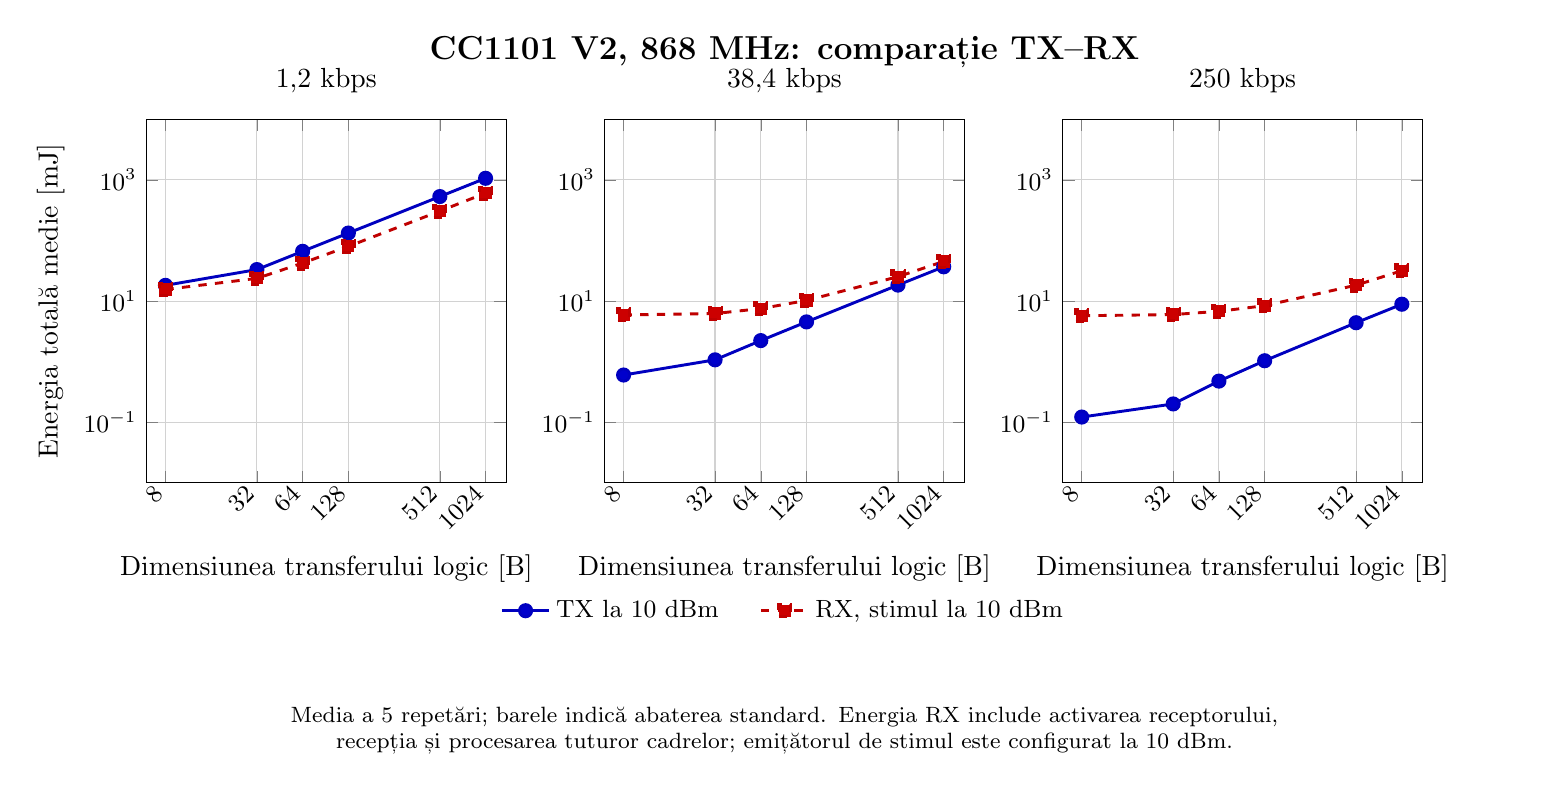
\begin{tikzpicture}
\begin{groupplot}[/pgf/number format/use comma,
  group style={group size=3 by 1, horizontal sep=1.25cm},
  width=6.15cm, height=6.2cm,
  xmode=log, log basis x={2},
  ymode=log, log basis y={10},
  ymin=0.01, ymax=10000,
  xmin=6, xmax=1400,
  xtick={8,32,64,128,512,1024},
  xticklabels={8,32,64,128,512,1024},
  x tick label style={rotate=45, anchor=east, font=\small},
  y tick label style={font=\small},
  grid=both, minor grid style={gray!15}, major grid style={gray!35},
  xlabel={Dimensiunea transferului logic [B]},
  every axis plot/.append style={line width=1.05pt},
  error bars/error bar style={line width=0.35pt},
  legend style={font=\small, draw=none, fill=none,
    at={(0.5,-0.29)}, anchor=north, legend columns=3,
    /tikz/every even column/.append style={column sep=0.45cm}},
]
\nextgroupplot[title={1{,}2 kbps}, ylabel={Energia totală medie [mJ]}]
\addplot+[
  color=blue!75!black, solid, mark=*, mark size=2.2pt,
  error bars/.cd, y dir=both, y explicit,
] coordinates {
  (8,18.1883048) +- (0,0.0177717961)
  (32,33.1117291) +- (0,0.0183400067)
  (64,66.2888726) +- (0,0.0194064677)
  (128,132.58372) +- (0,0.0251988428)
  (512,530.491757) +- (0,0.151785874)
  (1024,1061.48675) +- (0,0.313866891)
};
\addplot+[
  color=red!75!black, dashed, mark=square*, mark size=2.2pt,
  error bars/.cd, y dir=both, y explicit,
] coordinates {
  (8,15.5590016) +- (0,0.102233922)
  (32,23.6859387) +- (0,0.0784763647)
  (64,42.4202167) +- (0,0.129885331)
  (128,79.8934697) +- (0,0.112253916)
  (512,305.032136) +- (0,0.251286818)
  (1024,604.870649) +- (0,0.296795297)
};
\nextgroupplot[title={38{,}4 kbps}]
\addplot+[
  color=blue!75!black, solid, mark=*, mark size=2.2pt,
  error bars/.cd, y dir=both, y explicit,
] coordinates {
  (8,0.602501373) +- (0,0.00267156186)
  (32,1.07354411) +- (0,0.00317321951)
  (64,2.2285692) +- (0,0.006435654)
  (128,4.53645395) +- (0,0.00376653717)
  (512,18.3660392) +- (0,0.010287699)
  (1024,36.7936547) +- (0,0.00554884912)
};
\addlegendentry{TX la 10 dBm}
\addplot+[
  color=red!75!black, dashed, mark=square*, mark size=2.2pt,
  error bars/.cd, y dir=both, y explicit,
] coordinates {
  (8,5.90454187) +- (0,0.0539646164)
  (32,6.23293538) +- (0,0.033837558)
  (64,7.51688412) +- (0,0.144957039)
  (128,10.2473231) +- (0,0.0605734597)
  (512,25.296038) +- (0,0.0774512548)
  (1024,45.0424261) +- (0,0.149732149)
};
\addlegendentry{RX, stimul la 10 dBm}
\nextgroupplot[title={250 kbps}]
\addplot+[
  color=blue!75!black, solid, mark=*, mark size=2.2pt,
  error bars/.cd, y dir=both, y explicit,
] coordinates {
  (8,0.122087858) +- (0,0.0020178284)
  (32,0.2008944) +- (0,0.000923412057)
  (64,0.478253901) +- (0,0.0032034274)
  (128,1.03680708) +- (0,0.00397707218)
  (512,4.39720427) +- (0,0.00166498845)
  (1024,8.87376302) +- (0,0.00901416598)
};
\addplot+[
  color=red!75!black, dashed, mark=square*, mark size=2.2pt,
  error bars/.cd, y dir=both, y explicit,
] coordinates {
  (8,5.73147803) +- (0,0.0858621987)
  (32,5.98953795) +- (0,0.0280532689)
  (64,6.78052784) +- (0,0.050702048)
  (128,8.39435084) +- (0,0.110844111)
  (512,18.3127977) +- (0,0.118459231)
  (1024,31.6946818) +- (0,0.184063783)
};
\end{groupplot}
\node[font=\bfseries\large] at ($(group c2r1.north)+(0,0.85cm)$)
  {CC1101 V2, 868 MHz: comparație TX--RX};
\node[font=\footnotesize, align=center, text width=18.5cm]
  at ($(group c2r1.south)+(0,-3.15cm)$)
  {Media a 5 repetări; barele indică abaterea standard. Energia RX include activarea receptorului,\\
   recepția și procesarea tuturor cadrelor; emițătorul de stimul este configurat la 10 dBm.};
\end{tikzpicture}
\end{document}
